\documentclass[9pt]{extarticle}

\usepackage[utf8]{inputenc}              % Tipos de caracteres
\usepackage[portuguese]{babel}           % Português
\usepackage[a4paper,portrait]{geometry}  % Tipo de papel
\usepackage{color}                       % Para tratamento da cor
\usepackage{graphicx}                    % Para a imagem
\DeclareGraphicsExtensions{.jpg,.png}
\usepackage{amsmath}                     % Para as matematiquices
\usepackage{amssymb}
\usepackage{array}
\usepackage{gensymb}                     % Grau
\usepackage{multicol}
\setlength{\columnsep}{1cm}
\usepackage{geometry}					% Margens
%\usepackage{xfrac}
\usepackage{colortbl}

\usepackage{multirow}

\addtolength{\topmargin}{-28mm}
\addtolength{\textheight}{68mm}
\addtolength{\oddsidemargin}{-25mm}
\addtolength{\textwidth}{52mm}

\renewenvironment{abstract}
 {\small
  \begin{center}
  \bfseries \abstractname\vspace{-.5em}\vspace{0pt}
  \end{center}
  \list{}{
    \setlength{\leftmargin}{0cm}%
    \setlength{\rightmargin}{\leftmargin}%
  }%
  \item\relax}
 {\endlist}
 
\renewcommand{\abstractname}{Resumo}

\renewcommand{\refname}{Bibliografia}

\delimitershortfall-1sp
\newcommand\abs[1]{\left|#1\right|}
\newcommand{\PR}[1]{\ensuremath{\left[#1\right]}}
\newcommand{\PC}[1]{\ensuremath{\left(#1\right)}}
\newcommand{\chav}[1]{\ensuremath{\left\{#1\right\}}}

\newcolumntype{x}[1]{>{\centering\hspace{0pt}}p{#1}}

\begin{document}

\title {\bf \huge Estudo da Radiação Emitida por um Corpo Negro}
\author
{{\small João Ferreira (78179), Henrique Rodrigues (78632), Rodrigo C. Carvalho (78646) e Cristina Melício (78947)} \\
{\small MEFT $\cdot$ 2ºAno, 2º Semestre $\cdot$ Laboratório de Complementos de Eletromagnetismo e Termodinâmica}}
\date{{\small Grupo III $\cdot$ Sexta-Feira $\cdot$ 27 de Março de 2015}}
\maketitle

\begin{abstract}  
\par Nesta experiência foi estudada a emissão de radiação por diversos corpos enquanto aproximação do modelo de Corpo Negro. Verificou-se experimentalmente a Lei de Planck e a Lei de Wien com o auxílio de uma lâmpada de tungsténio para três temperaturas distintas, tendo sido obtido para a constante de Wien o valor de $(2.5\pm0.4)m\cdot K$. Posteriormente, determinou-se o expoente da temperatura na lei de Stefan, tendo-se verificado que este correspondia a $\alpha=4.64\pm0.02$. Por fim, comparam-se as emissividades de diferentes faces de um cubo de Leslie.
\end{abstract}

\begin{multicols}{2}

\section{Introdução}

\par Esta experiência consiste no estudo de um corpo negro, que é definido como sendo um corpo que absorve toda a radiação que nele incide sem a refletir ou transmitir inteiramente, irradiando posteriormente de acordo com a sua temperatura absoluta $T$.

\par Para um corpo arbitrário define-se o seu poder de absorção como sendo:
\begin{equation}
Q = \frac{P_a}{P_i}
\end{equation}
\begin{center}
\par\noindent {\scriptsize(onde $P_a$ é a potência absorvida e $P_i$ é a potência incidente)}
\end{center}
\par Para o corpo negro tem-se que $Q_N = 1$ uma vez que absorve toda a radiação que nele incide e para os outros corpos tem-se $Q_C < 1$ .
\par A emissividade é dada pelo quociente:
\begin{equation}
e = \frac{Q_C}{Q_N}
\end{equation}
\par Sendo assim, para o corpo negro $e_N = 1$ e para os outros corpos $e_C < 1$.

\par O comportamento de um corpo relativamente à radiação emitida é descrito pelo poder emissivo ou emitância $I_C$ e é caracterizado como sendo a energia radiada por unidade de tempo e por unidade de área em todos os comprimentos de onda. É possível quantificar o poder emissivo do corpo negro $I_N$ pela Lei de radiação de Stefan \footnote{$\sigma=5.6697\times10^{-8}Wm^{-2}K^{-4}$ é constante de Stefan}
\begin{equation} \label{stefan}
I_N = \sigma T^4
\end{equation}  

\par Tem-se assim o Teorema de Kirchoff que considera a relação entre o poder emissivo e o poder de absorção como sendo:
\begin{equation}
F(T) = \frac{I_C}{Q_C} = \sigma T^4
\end{equation}
\par Deste enunciado, conclui-se que a emissividade e o poder de absorção são iguais, sendo que um bom absorsor é um bom emissor e vice versa. Utilizaremos um cubo de Leslie

\par A partir de lei de Stefan, conclui-se que a emissão de radiação por um corpo negro depende apenas da sua temperatura, quando este se encontra em equilíbrio térmico. Tem-se então a Lei de Wien, segundo a qual quanto maior for a temperatura $T$ de um corpo negro menor é o comprimento de onda $\lambda_{max}$ correspondente ao poder emissivo máximo\footnote{$b=2.8977685\times10^{-3}m\cdot K$ é a constante de dispersão de Wien}:
\begin{equation} \label{wien}
\lambda_{max} T = b
\end{equation}

\par A intensidade da radiação de um dado comprimento de onda $\lambda$ emitida por um corpo negro a uma temperatura absoluta $T$ é dada pela Lei de radiação de Planck:
\begin{equation} \label{planck}
I_{(T,\lambda)} = \frac{2h\pi c^2}{\lambda^5} \PC{e^{\frac{hc}{\lambda k_B T}}-1}^{-1}
\end{equation}
\begin{center}
\par\noindent {\scriptsize(em que $h$ é a constante de \textit{Planck}, $k_B$ a constante de \textit{Boltzmann} e $c$ a velocidade da luz)}
\end{center}

%\par É de realçar ainda que, no que toca ao cubo de Leslie, verifica-se que a diferença de tensão gerada pelo detector seria directamente proporcional à intensidade de radiação que sobre ele incide apenas no caso de ele próprio se encontrar a uma temperatura correspondente ao zero absoluto. Todavia, tal não é verdade. De facto, ele irá emitir radiação segundo a lei de Stefan-Boltzmann previamente enunciada. Assim, sabemos que a diferença de potencial gerada será na realidade proporcional à intensidade de radiação emitida pelo detector menos a que sobre ele incide. Sabendo que a temperatura do sensor é quase igual à da temperatura da sala (visto este se encontrar protegido da radiação que sobre ele incide excepto aquando do momento de fazer medições), temos que

%\begin{equation}
%V \propto (T^4-T_{det}^4)
%\end{equation}
%\begin{center}
%\par\noindent {\scriptsize(em que $V$ é a diferença de potencial medida, $T$ a Temperatura a que se encontra o emissor de radiação e $T_det$ a temperatura do detector)}
%\end{center}


\section{Montagem da Experiência}
\subsection{Lei de Planck e Lei de Wien}
\par Na primeira parte da experiência, cujo objetivo é a obtenção do espectro de emissão de um modelo do corpo negro, o esquema da montagem está representado na figura 1.

\begin{center}
\includegraphics[width=180pt]{parte1.jpg}
\begin{center}
\par\noindent {\scriptsize ({\bf Figura 1}:Esquema da montagem da primeira parte)}
\end{center}
\end{center}

\par O modelo de corpo negro usado para esta parte é uma lâmpada de filamento de tungsténio cuja tensão máxima é $13 V$, sendo, por isso, colocados um voltímetro em paralelo, e um amperímetro em série, de forma a controlar a tensão e a corrente no circuito. Além disso, a resistência em série serve para evitar sobrecargas no circuito de alimentação.

\par Tem-se então um goniómetro, associado a um prisma de dispersão, composto por dois braços: o braço fixo que recebe a radiação da fonte e a faz incidir sobre o prisma e o braço móvel que recebe do prisma a radiação refratada e a faz incidir no detetor. O detetor da radiação utilizado é uma termopilha com resposta uniforme na gama compreendida entre os $500 nm$ e os $25000 nm$, ou seja, da radiação verde à infravermelha, que funciona por efeito de \textit{Peltier} devido à diferença de temperatura entre os sensores do início e do fim do detetor.
\par O esquema do prisma de dispersão e dos seus ângulos encontra-se na figura 2.

\begin{center}
\includegraphics[width=180pt]{prisma.jpg}
\begin{center}
\par\noindent {\scriptsize ({\bf Figura 2}: Esquema do prisma de dispersão. Devido à geometria equilátera da base do prisma, $\alpha=60^\circ$)}
\end{center}
\end{center}

\subsection{Verificação da Lei de \textit{Stefan}}
\par Na segunda parte da experiência, retirou-se o goniómetro e o prisma, e colocou-se a uma distância fixa a lâmpada na direção do detetor. O esquema da montagem está na figura 3.

\vspace{-1cm}

\begin{center}
\includegraphics[width=180pt]{parte2.jpg}
\begin{center}
\par\noindent {\scriptsize ({\bf Figura 3}: Esquema da montagem da segunda parte)}
\end{center}
\end{center}

\subsection{Cubo de Leslie}
Na terceira parte da experiência utiliza-se um Cubo de \textit{Leslie} constituído por quatro faces com diferentes revestimentos exteriores: preta, espelhada, branca e metálica. O esquema da montagem está na figura 4.

\begin{center}
\includegraphics[width=180pt]{parte3.jpg}
\begin{center}
\par\noindent {\scriptsize ({\bf Figura 4}: Esquema da montagem da terceira parte)}
\end{center}
\end{center}


\section{Dados Experimentais}

\subsection{Lei de Planck e Lei de Wien}

\par Efectuou-se a montagem da figura 1 apresentada anteriormente. De seguida, alinhou-se o goniómetro. Para tal, foi necessário em primeiro lugar colocar a máscara com fenda vertical sobre a lente de saída de radiação, rodar a plataforma onde está colocado o prisma e medir o ângulo $\theta_1$ para o qual o feixe refletido pela face do prisma coincide com o feixe nela incidente. Depois, sem a máscara, rodar essa mesma plataforma no sentido anti-horário, observar o espectro num alvo (a parede) e registar o ângulo $\theta_2$ correspondente ao desvio mínimo\footnote{Cada uma destas medições foi efetuada separadamente pelos quatro elementos do grupo, tendo-se considerado a média entre eles.}. Fixou-se a posição angular do prisma e calculou-se o ângulo $\theta$ de incidência da radiação no prisma efetuando a diferença $\theta= \theta_1-\theta_2$. Obteve-se o seguinte valor:

\begin{center}
\begin{tabular}{ x{1cm} x{2cm} }
\hline \hline
$\theta$ $(^\circ)$ & 43.3$\pm$0.4 \tabularnewline
\hline \hline
\end{tabular}
\end{center}

\par Ajustou-se a tensão da fonte para $12V$. Retiraram-se as coberturas do braço do detetor e da sua entrada. Rodou-se este braço até que nele incidisse a radiação verde e registou-se este ângulo $\delta'$. Colocaram-se novamente ambas as coberturas, ligou-se o microvoltímetro, e anulou-se a sua leitura. Retirou-se agora a cobertura da entrada, mediu-se o valor indicado no microvoltímetro, e colocou-se novamente a cobertura. Fizeram-se mais duas medições, tendo o cuidado de verificar que com a cobertura colocada o valor indicado no microvoltímetro não ultrapassava os $3\mu V$. Rodou-se então o braço do detetor em intervalos angulares de $20'$ e $40'$ de modo a obter medições para 20 posições angulares $\delta'$ diferentes, registando-se para cada uma três valores de tensão lidos no microvoltímetro, cuja média corresponde ao valor $V$. Efetuaram-se medições numa maior densidade perto do máximo de intensidade luminosa, por forma a encontrar a sua posição angular.

\par Repetiu-se este procedimento para tensões da fonte de $9V$ e $6V$. Para cada tensão $V_f$, registou-se a intensidade de corrente $I$ que percorre a lâmpada e calculou-se a resistência $R$ pela lei de Ohm:

\begin{equation}
R=\frac{V_f}{I}
\end{equation}

\par A temperatura $T$ do filamento foi obtida por interpolação linear da tabela \verb|tab2.pdf|\footnote{\label{note1}Tabela disponibilizada pelo docente na página da cadeira} do valor de $\frac{R}{R_0}$, em que $R_0=0.4911$ é o conhecido para a temperatura $T=292.35K$. Obtiveram-se as seguintes temperaturas:

\begin{center}
\begin{tabular}{ x{2cm} x{2cm} }
$V_f$ $(V)$ & $T$ $(K)$ \tabularnewline
\hline \hline
$12.02\pm0.01$ & $2404\pm12$ \tabularnewline
$9.00\pm0.01$ & $2130\pm13$ \tabularnewline
$5.97\pm0.01$ & $1877\pm16$ \tabularnewline
\end{tabular}
\par\noindent {\scriptsize ({\bf Tabela 1}: Valores das temperaturas de trabalho para as diferentes tensões da fonte)}
\end{center}

\par No final, o docente removeu o prisma de dispersão, e mediu-se o ângulo $\gamma$ correspondente ao alinhamento direto entre os braços do goniómetro, tendo-se obtido o seguinte valor:

\begin{center}
\begin{tabular}{ x{1cm} x{2cm} }
\hline \hline
$\gamma$ $(^\circ)$ & 274.00$\pm$0.01 \tabularnewline
\hline \hline
\end{tabular}
\end{center}

\par Os valores angulares $\delta$ que se utilizaram na análise subsequente dos resultados foram obtidos através da diferença $\delta=\gamma-\delta'$.

\par Para cada valor de $\delta$, obteve-se um valor de indíce de refração $n$, dado pela seguinte expressão:

\begin{equation} \label{eq:n}
n=\sqrt{\PC{\sin^2{\theta}}+ \PC{\frac{\sin{\PC{\delta-\theta+\alpha}}+ \cos{\alpha}\sin{\theta}}{\sin{\alpha}}}^2}
\end{equation}

\par Para cada valor de indíce de refração $n$, efetuou-se uma interpolação linear dos valores da tabela \verb|tab1.jpg|\footnotemark[\ref{note1}] referente à curva de dispersão do prisma utilizado para obter os vários comprimentos de onda $\lambda$ correpondentes.

\par Na figura 5 apresentam-se os valores da intensidade luminosa, obtidos a partir da normalização dos valores de tensão medidos anteriormente, como função do comprimento de onda da radiação incidente - $I(\lambda)$ -, para as três temperaturas diferentes. A estes pontos ajustou-se  equação \eqref{planck}.

\begin{equation} \label{planckP}
I(\lambda) = \frac{2\pi hc^2}{\PC{\lambda-c_1}^5} \PC{e^{\frac{hc}{k_BT\PC{\lambda-c_1}}}-1}^{-1}\frac{1}{d}
\end{equation}
\begin{center}
\par\noindent {\scriptsize onde $d$ é uma constante de normalização dada por:
\begin{equation}
d=\frac{2\pi hc^2T^5}{b^5} \PC{e^{\frac{hc}{k_Bb}}-1}^{-1}
\end{equation}
\end{center}

\begin{center}
\includegraphics[width=180pt]{espetro1.pdf}
\includegraphics[width=180pt]{espetro2.pdf}
\includegraphics[width=180pt]{espetro3.pdf}
\par\noindent {\scriptsize ({\bf Figura 5}: Intensidade luminosa em função do comprimento de onda. A vermelho indicam-se os pontos $(756nm,0.485)$ e $(1583nm,0.750)$ no primeiro gráfico, $(801nm,0.492)$ e $(1915nm,0.623)$ no segundo gráfico e $(980nm,0.643)$ e $(1549nm,0.940)$ no terceiro gráfico. A azul, roxo e amarelo, representam-se os ajustes da equação \eqref{planckP} pelo método dos mínimos quadrados para as diferentes temperaturas, e a verde as curvas teóricas respetivas.)}
\end{center}

%\begin{center}
%\includegraphics[width=240pt]{espetro3.pdf}
%\par\noindent {\scriptsize ({\bf Gráfico 3}: Intensidade luminosa em função do comprimento de onda, para $T=1887K$. A vermelho indicam-se os pontos $(,nm)$ e $(,nm)$). A azul representa-se o ajuste da equação \eqref{planckP} pelo método dos mínimos quadrados, e a verde a curva teórica para esta temperatura.)}
%\end{center}

\pagebreak

\par Obtiveram-se os seguintes parâmetros de ajuste:

{\small
\begin{center}
\begin{tabular}{ x{1.1cm} x{2cm} x{2cm} x{2cm} }
 & $T=2404K$ & $T=2130K$ & $T=1877K$ \tabularnewline
\hline \hline
$c_1$ $(nm)$ & 143$\pm$22 & 149$\pm$24 & 123$\pm$24 \tabularnewline
\end{tabular}
\par\noindent {\scriptsize ({\bf Tabela 2}: Parâmetros resultantes do ajuste da equação \eqref{planckP} aos pontos dos diferentes gráficos da figura 5)}
\end{center}
}

\par Para as diferentes temperaturas, obtiveram-se os seguintes valores para o comprimento de onda correspondente ao máximo de intensidade luminosa:

{\small
\begin{center}
\begin{tabular}{ x{1.5cm} x{1.8cm} x{1.8cm} x{1.8cm} }
 & $T=2404K$ & $T=2130K$ & $T=1877K$ \tabularnewline
\hline \hline
$\lambda_{max}$ $(nm)$ & 1148$\pm$53 & 1319$\pm$70 & 1433$\pm$87 \tabularnewline
\end{tabular}
\par\noindent {\scriptsize ({\bf Tabela 3}: Comprimentos de onda correspondente ao máximo da intensidade luminosa, para as diferentes temperaturas)}
\end{center}
}

\subsection{Lei de Stefan}

\par Efetuou-se agora a montagem da figura 3, e mediu-se a intensidade da radiação emitida para diferentes valores de tensão da lâmpada. Obtiveram-se os seguintes resultados:

{\small
\begin{center}
\begin{tabular}{ x{2cm} x{2cm}}
$V_f(V)$ & $V(mV)$ \tabularnewline
\hline \hline
11.98$\pm$0.01  & 6.91$\pm$0.01 \tabularnewline
10.99$\pm$0.01  & 6.07$\pm$0.01 \tabularnewline
9.95$\pm$0.01   & 5.16$\pm$0.01 \tabularnewline
9.00$\pm$0.01   & 4.35$\pm$0.01 \tabularnewline
7.99$\pm$0.01   & 3.55$\pm$0.01 \tabularnewline
7.02$\pm$0.01   & 2.86$\pm$0.01 \tabularnewline
5.99$\pm$0.01   & 2.16$\pm$0.01 \tabularnewline
5.02$\pm$0.01   & 1.56$\pm$0.01 \tabularnewline
3.995$\pm$0.001 & 1.03$\pm$0.01 \tabularnewline
2.897$\pm$0.001 & 0.57$\pm$0.01 \tabularnewline
\end{tabular}
\par\noindent {\scriptsize ({\bf Tabela 4}: Comprimentos de onda correspondente ao máximo da intensidade luminosa, para as diferentes temperaturas)}
\end{center}
}

\subsection{Cubo de Leslie}

\par Efetuou-se a montagem da figura 4 e estudou-se a emissividade das diversas faces do cubo. Ligou-se a fonte de tensão e esperou-se que a temperatura $T$ das faces do cubo estabilizasse, tendo-se registado este valor. De seguida, mediu-se a intensidade da radiação emitida por cada face do cubo. Consideraram-se duas temperaturas distintas, tendo-se obtidos os seguintes resultados:

{\small
\begin{center}
\begin{tabular}{ x{2.2cm} x{2cm} x{2cm} }
Face & $T=(90\pm1)^\circ C$ & $T=(69\pm1)^\circ C$ \tabularnewline
\hline \hline
$V_{\text{Preta}}$ $(mV)$ & 12.43$\pm$0.01 & 7.07$\pm$0.01 \tabularnewline
$V_{\text{Espelhada}}$ $(mV)$ & 0.66$\pm$0.01 & 0.26$\pm$0.01 \tabularnewline
$V_{\text{Branca}}$ $(mV)$ & 12.46$\pm$0.01 & 6.96$\pm$0.01 \tabularnewline
$V_{\text{Metálica}}$ $(mV)$ & 3.46$\pm$0.01 & 1.82$\pm$0.01 \tabularnewline
\end{tabular}
\par\noindent {\scriptsize ({\bf Tabela 5}: Intensidade da radiação emitida por cada face do cubo, para diferentes temperaturas)}
\end{center}
}

%\par Por fim, foi efectuado um processo adicional de medir o valor do expoente da relação de Stefan, utilizando o raciocínio delineado nos últimos parágrafos da introdução. Considerando a face espelhada, fez-se variar a temperatura do cubo de Leslie, medindo-se para cada uma o valor da tensão indicada no sensor. Obtiveram-se os seguintes resultados:

%{\bf ESTES VALORES NAO FAZEM SENTIDO, VAO VER O EXCELL. POR MIM NAO SE POE}

%{\small
%\begin{center}
%\begin{tabular}{ x{2cm} x{2cm} }
%$T$ $(^\circ C)$ & $V$ $(mV)$ \tabularnewline
%\hline \hline
%41$\pm$1 & 0.23$\pm$0.01 \tabularnewline
%49$\pm$1 & 0.36$\pm$0.01 \tabularnewline
%56$\pm$1 & $\pm$0.01 \tabularnewline
%63$\pm$1 & $\pm$0.01 \tabularnewline
%72$\pm$1 & $\pm$0.01 \tabularnewline
%77$\pm$1 & $\pm$0.01 \tabularnewline
%85$\pm$1 & $\pm$0.01 \tabularnewline
%\end{tabular}
%\par\noindent {\scriptsize ({\bf Tabela 5}: Tensão detetada pelo sensor, referente à intensidade da radiação emitida pela face espelhada, para diferentes temperaturas)}
%\end{center}
%}

\section{Discussão dos Resultados}

\subsection{Lei de Planck e Lei de Wien. Eficiência da lâmpada}

\par Relativamente à primeira parte da experiência, efectuou-se o ajuste experimental dos dados obtidos à lei de Planck. Todavia, verificou-se que os dados apresentavam uma translação em relação ao máximo, fruto de um erro sistemático existente na experiência. Por conseguinte, efectuou-se um ajuste do tipo $x-c_1$, verificando-se uma muito melhor aproximação dos dados experimentais ao fit efectuado, existindo concordância a nível do máximo em relação a previsão teórica (tal como foi apresentado na secção anterior) e apenas começando a verificar-se desvios significativos a partir de cerca de $3000nm$. É possível ver a sobreposição dos gráficos para as diversas temperaturas consideradas na figura 6:

\begin{center}
\includegraphics[width=180pt]{espetroT.pdf}
\par\noindent {\scriptsize ({\bf Figura 6}: Intensidade luminosa em função do comprimento de onda para as três temperaturas diferentes, normalizados de acordo com o máximo da mais elevada. A vermelho indicam-se os pontos $(756nm,0.485)$ e $(1583nm,0.750)$ no gráfico azul, $(801nm,0.287)$ e $(1915nm,0.363)$ no gráfico roxo, e $(980nm,0.217)$ e $(1549nm,0.318)$ no gráfico amarelo.)}
\end{center}

\par Relativamente à eficiência da lâmpada, esta foi tomada mediante a integração numérica das curvas obtidas para a Lei de Planck para cada diferente temperatura, tendo-se utilizado o método dos trapézios. Para estimar o erro inerente ao método, integrou-se o erro também mediante o método dos trapézios, obtendo por conseguinte um majorante válido. Assim, foi possível obter os seguintes resultados, tendo em conta que o valor teórico $\epsilon_t$ foi previsto pelo software \verb|Mathematica|:

{\small
\begin{center}
\begin{tabular}{ x{1.1cm} x{2cm} x{2cm} x{2cm} }
 & $T=2404K$ & $T=2130K$ & $T=1877K$ \tabularnewline
\hline \hline
$I_{\text{total}}$ & $17.7\pm0.12$ & $10.4\pm0.08$ & $6.2\pm0.1$ \tabularnewline
$I_{\text{visivel}}$ & $0.502\pm0.005$ & $0.171\pm0.004$ & $0.048\pm0.004$ \tabularnewline
$\epsilon$ $(\%)$ & $2.92\pm0.02$ & $1.64\pm0.04$ & $0.78\pm0.06$ \tabularnewline
$\epsilon_t$ $(\%)$ & $3.9$ & $1.95$ & $0.84$ \tabularnewline
\end{tabular}
\par\noindent {\scriptsize ({\bf Tabela 6}: Eficiência para diferentes temperaturas)}
\end{center}
}

\par= De facto, foi possível obter o valor da eficiência em função da temperatura ajustando a equação seguinte, onde a função f se refere à intensidade luminosa em função da lei de Planck

\begin{equation}
\epsilon=}\frac{\int_{370nm}^{750nm} f(\lambda,T)d\lambda}{\int_0^\infty f(\lambda,T)d\lambda}
\end{equation}

\par Assim, obteve-se um gráfico para a eficiência em função da temperatura, apresentado na figura 7:

\begin{center}
\includegraphics[width=180pt]{calculoeficiencia.pdf}
\par\noindent {\scriptsize ({\bf Figura 7}: Gráfico da eficiência da lâmpada como função da temperatura do seu filamento, obtido com o software \verb|Mathematica|)}
\end{center}

\par Verificou-se que o máximo ocorreu a $T=7138K$, com um valor de $\epsilon=48.3\%$ pelo que nos encontramos assim aquando da realização da experiência num domínio de eficiências muito baixo. Além disso, notamos que quão menor a temperatura, maior a concordância entre o valor teórico e o valor experimental. Devemos no entanto realçar que existe ainda uma diferença significativa entre a eficiência de um corpo negro e a da lâmpada, que resulta naturalmente de esta não ser exactamente um corpo negro bem como de ruído inerente à realização da experiência - esta não foi feita na ausência total de luz ambiente, por exemplo.

\par Analisemos os valores da tabela 3. Representa-se no gráfico da figura 8 o comprimento de onda correspondente ao máximo de intensidade $\lambda_{max}$ em função do inverso da temperatura. A estes pontos ajustou-se a seguinte reta, relacionada com a lei de Wien \eqref{wien}:

\begin{equation} \label{wienP}
\lambda_{max}\PC{T^{-1}}=\PC{\beta T^{-1}+\alpha}\times10^{9}
\end{equation}

\begin{center}
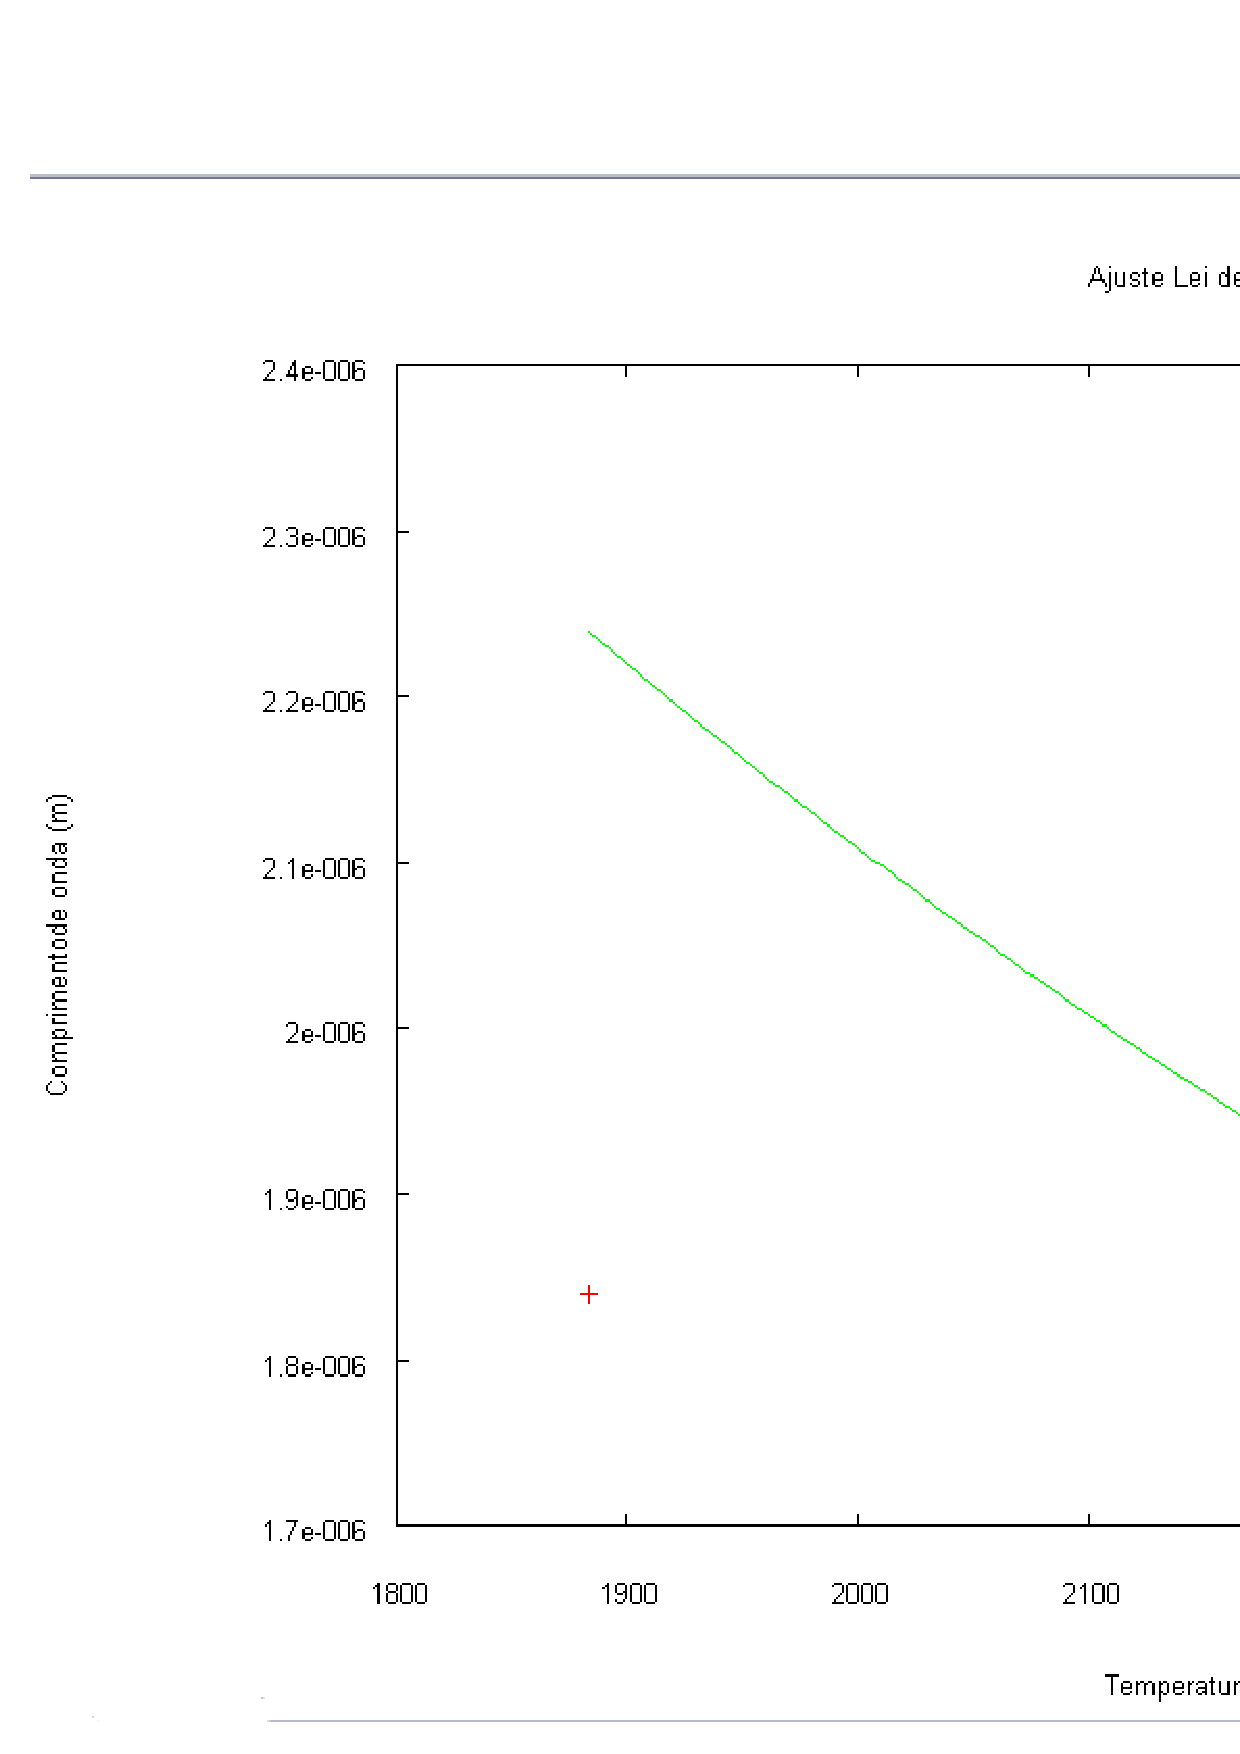
\includegraphics[width=180pt]{wien.pdf}
\par\noindent {\scriptsize ({\bf Figura 8}: Gráfico da verificação experimental da lei de Wien. A azul representa-se o ajuste da equação \eqref{wienP} pelo método dos mínimos quadrados)}
\end{center}

\par Obtiveram-se os seguintes parâmetros de ajuste:

{\small
\begin{center}
\begin{tabular}{ x{1.5cm} x{2.4cm} }
\hline \hline
$\alpha$ $(m)$ & $\PC{1\pm2}\times10^{-7}$ \tabularnewline
$\beta$ $(m\cdot K)$ & $\PC{2.5\pm0.4}\times10^{-3}$ \tabularnewline
\hline \hline
\end{tabular}
\end{center}
}

\par Obteve-se então um valor para a constante de dispersão de Wien que apresenta um desvio à exactidão de $14\%$ e um desvio à precisão de $15\%$. Devemos realçar que, apesar da boa qualidade do valor obtido, esta poderia ser largamente melhorada utilizando um maior número de temperaturas e comprimentos de onda a partir dos quais obter esta constante - de facto, apenas foram estudados 3 pares $(\lambda,T)$.

\subsection{Lei de Stefan}

\par Analisemos os valores da tabela 4. Para cada tensão da fonte, foi possível o valor da temperatura $T$ do filamento correspondente, pelo método utilizado anteriormente, com o auxílio da tabela \verb|tab2.pdf|. Na figura 9 representa-se o gráfico do logaritmo dos valores detetados pelo sensor como função do logaritmo da temperatura, aos quais se ajustou a seguinte equação, relacionada com a lei de Stefan \eqref{stefan}:

\begin{equation} \label{stefanP}
\log(V)=\alpha\log(T)+\beta
\end{equation}

\begin{center}
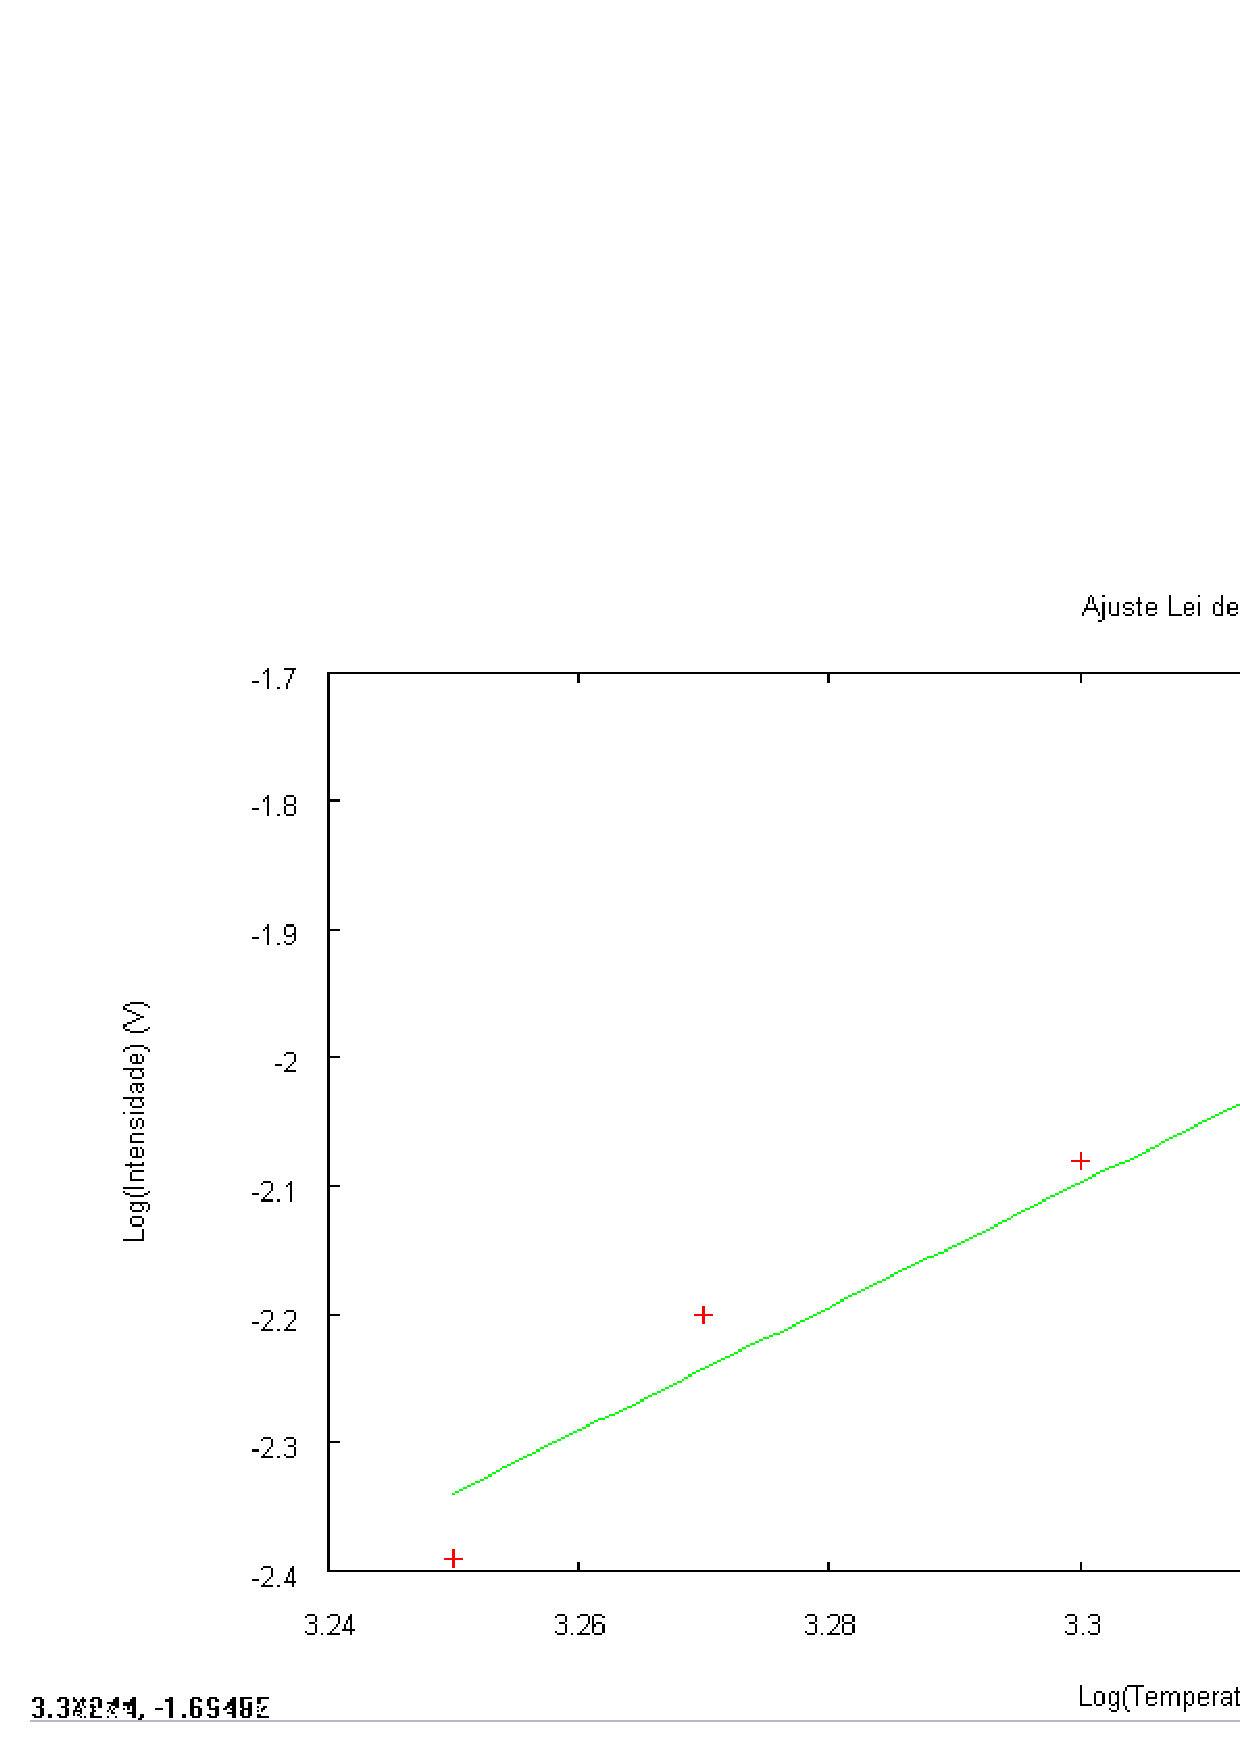
\includegraphics[width=180pt]{stefan.pdf}
\par\noindent {\scriptsize ({\bf Figura 9}: Gráfico da verificação experimental da lei de Stefan. A azul representa-se o ajuste da equação \eqref{stefanP} pelo método dos mínimos quadrados)}
\end{center}

\par Obtiveram-se os seguintes parâmetros de ajuste:

{\small
\begin{center}
\begin{tabular}{ x{1.2cm} x{2.4cm} }
\hline \hline
$\alpha$ & 4.64$\pm$0.02 \tabularnewline
$\beta$  & -17.84$\pm$0.05 \tabularnewline
\hline \hline
\end{tabular}
\end{center}
}

\par Obteve-se então como expoente na lei de Stefan o valor $\alpha=4.64\pm0.02$. De facto, notamos que existe uma discrepância acentuada entre este valor e o expectável teórico, verificando-se um desvio à exactidão de $16\%$ e um desvio à precisão de $4.3\%$. Poderíamos erroneamente considerar que tal resulta do facto de não se tratar de um corpo negro - todavia, isto deveria reflectir-se na constante multiplicativa relativa à emissividade e, por conseguinte, apesar de influir de certo modo, nunca alteraria de forma tão significativa o valor do expoente. De facto, este valor é lógico tendo em conta que não existia um isolamento perfeito - a saber, sobre o detector incidiriam naturalmente radiações provenientes dos membros do grupo na sala, dos dispositivos electrónicos que com eles estavam, entre outras. Logo, é natural que o valor do expoente seja superior porque a radiação detectada foi de facto superior àquela que seria suposto incidir sobre o detector. Devemos ainda notar que os gráficos experimentais para a intensidade em função do comprimento de onda apresentam um declive superior ao teórico. Partindo do pressuposto que a emissivididade da fonte de radiação se manteve constante, tal resultaria unicamente de uma variação no expoente - evidenciado agora nesta parte da experiência.

\subsection{Cubo de Leslie}

\par Quanto aos resultados da tabela 5, sabemos que, quanto maior for o valor de intensidade verificado, de acordo com o Teorema de Kirchoff, mais elevada será a emissividade da face à qual pertence esse valor - sendo que esta será por conseguinte uma melhor emissora de radiação, absorvendo também uma maior quantidade da radiação que sobre ela incide. Assim, pela análise dos resultados, facilmente se depreende que a face com a maior emissividade será a face negra, tal como esperado, e que a de menor emissividade (melhor reflectora) será a espelhada. Todavia, no tocante  às restantes faces, notamos uma discrepância - a branca apresenta um valor quase idêntico ao da face negra, enquanto que a metálica se comporta como esperado e apresenta um valor demarcadamente inferior. Isto é facilmente explicável - uma face metálica reflecte a radiação visível. Todavia, nada sabemos quanto à emissividade do material que  ca onstitui no tocante a quaisquer outros comprimentos de onda. Ora, considerando que a zona visível do espectro constituiu uma ínfima parte da emissão da lâmpada - e não aquela para a qual possui o seu máximo de intensidade de emissão - podemos concluir que o material de que esta face é constituída é reflectivo na zona do visível mas possui uma muito elevada emissividade para outras zonas, nomeadamente a do infravermelho. Tal como antecipado, notamos igualmente que quão maior for a temperatura, maior será a intensidade da radiação emitida.

\section{Conclusões}

\par Após efectuar a experiência é possível constatar que existem diversos erros associados à execução da própria e que não são elimináveis - interpolação linear dos dados da tabela dos indíces de refracção, ruído electromagnético de fundo, a sensibilidade do aparelho de medição que flutua entre diversos valores de diferença de potencial, entre outros - e que comprometem a qualidade das medições efectuadas, não sendo inteiramente suprimidos pela execução de diversas medidas para cada valor estudado. Todavia, é de notar que os resultados em si se encontram razoáveis, verificando-se que na primeira parte após a translação efectuada existe uma concordância razoável entre os máximos teóricos e experimentais; um valor para a constante de Wien que se encontra dentro da incerteza experimental; um expoente para a Lei de Stefan-Boltzmann razoável tendo em conta as limitações da aproximação efectuada e, por fim, os resultados previstos teoricamente para o cubo de Leslie verificam-se experimentalmente.

\begin{thebibliography}{9}

\bibitem{guia} Guia de objetivos do trabalho, Professor João Figueirinhas
\bibitem{apontamentos} Apontamentos das aulas teóricas
\bibitem{utilizador} Thermal Radiation System, PASCO scientific

%\bibitem{site} Wikipedia, the free encyclopedia - Thermoelectric effect. [Online] Available from: \url{http://en.wikipedia.org/wiki/thermoelectric\_effect}
\end{thebibliography}

\vfill

\pagebreak

%\section{Anexos}
%\subsection*{\normalsize Material}
%\begin{itemize}
%\item Cenas
%\end{itemize}
%
%\subsection*{\normalsize Tabelas Completas de Resultados}
%\par Cenas

\end{multicols}

\end{document}

% FOTOGRAFIA
%\begin{center}
%\includegraphics[width=240pt]{NOME SEM EXTENSAO}
%\par\noindent {\scriptsize (Figura X: Descrição)}
%\end{center}

%NOVA SUBSECÇÃO
%\subsection*{\normalsize BLA BLA}

%TABELA
%\begin{center}
%\begin{tabular}{ x{1.5cm} ... }
%i & ... \tabularnewline
%\hline \hline
%1 & 4.15  & 0.15  & 2033 & -  \tabularnewline
%\end{tabular}
%\par\noindent {\scriptsize (Tabela X: Descrição)}
%\end{center}
